\documentclass[a4paper,12pt]{article}
\usepackage[utf8]{inputenc}
\usepackage{graphicx} 
\usepackage{circuitikz}
\usepackage{fancyhdr} 
\usepackage{ragged2e}
\usepackage{amssymb}
\usepackage{blindtext} 
\usepackage{xcolor} 
\usepackage{url}
\usepackage[svgnames]{xcolor}
\usepackage{framed}
\usepackage{amsmath}
\usepackage{amsthm}
\usepackage{amssymb}
\usepackage{braket}
\usepackage{multicol}
\usepackage{graphicx}
\usepackage[export]{adjustbox}
\usepackage[table]{xcolor}
\usepackage{tabularx}
\usepackage[numbers]{natbib}
\usepackage{listings}
\usepackage{booktabs}
\usepackage{caption}
\captionsetup{font=small,labelfont=bf}
\captionsetup[table]{position=top,skip=8pt}
\captionsetup[figure]{skip=6pt}
\renewcommand{\arraystretch}{1.3}
\emergencystretch=1.5em
\usepackage{tikz}
\usepackage{lipsum} % Solo para texto de ejemplo

% Definición del estilo para el código
\lstdefinestyle{mipython}{
    language=Python,
    backgroundcolor=\color{lightgray!10},
    basicstyle=\ttfamily\small,
    breaklines=true,           % Rompe líneas largas automáticamente
    breakatwhitespace=true,    % Rompe solo en espacios (ideal para URLs)
    frame=single,              % Recuadro simple alrededor
    numbers=left,              % Números de línea
    numberstyle=\tiny\color{gray},
    captionpos=b,
    tabsize=4
}

\definecolor{shadecolor}{named}{LightGray}

\topmargin=-1cm
\oddsidemargin=0cm
\textheight=24cm
\textwidth=17cm

\usetikzlibrary{shapes.geometric} 
\usetikzlibrary{
    arrows.meta,
    decorations.pathmorphing,
    patterns, 
    calc
}  

\definecolor{shadecolor}{named}{LightGray}
\topmargin=-1cm
\oddsidemargin=0cm
\textheight=24cm
\textwidth=17cm

\begin{document}

\renewcommand{\tablename}{Tabla}
\renewcommand{\figurename}{Figura}

\begin{titlepage}

\begin{minipage}{2.6cm}

\includegraphics[width=\textwidth]{PNGs/ecfm.png}
\end{minipage}
\hfill
\begin{minipage}{6cm}
\begin{center}
\normalsize{Universidad de San Carlos de Guatemala\\
Escuela de Ciencias Físicas y Matemáticas\\ }
\end{center}
\end{minipage}
\hspace{0.5cm} 
\hfill
\begin{minipage}{2.6cm}

\includegraphics[width=\textwidth]{PNGs/usac.png}
\end{minipage}


\vspace{0.5cm} 

\begin{center}
\vspace{5.25cm}
\large{Informe Final}\\
\Large{\bf Aprendizaje de herramientas de Fermi-LAT para estudio de GRBs}\\


\vspace{4cm}

\normalsize
Fabricio C. Mencos \\
\vspace{0.5cm}
Supervisado por: \\
Dr. Rodrigo Sacahuí (ECFM-USAC) \\
\vspace*{4cm}
\small{Julio de 2026} \\

\vspace*{3cm}

\vspace{5cm}

\normalsize

\end{center}
\end{titlepage}



\newpage 
\renewcommand{\contentsname}{Índice}
\tableofcontents
\newpage

\section{Introducción}

Los estallidos de rayos gamma (Gamma-Ray Bursts, GRBs) son destellos intensos y breves, que durante unos pocos segundos, se vuelven la fuente electromagnética más energética y brillante del Universo \cite{Piran2000} en rayos X duros y gammas de hasta 100 MeV. La duración de estos puede variar desde algunos milisegundos hasta varios miles de segundos, el espectro de este fenómeno no es térmico y se describe con una componente de ley de potencias que se extiende desde cientos de keV hasta varios GeV. Estos fenómenos están asociados al colapso de estrellas masivas (largos) o a la fusión de objetos compactos (cortos) \cite{Rosswog2009}. 

\vspace{0.5cm}

 Los GRBs generan chorros relativistas en donde se aceleran partículas, principalmente electrones, que radian emisión sincrotrón en condiciones donde la densidad y el campo magnético son extremos. Debido a su enorme luminosidad y a esas condiciones físicas tan extremas, los GRBs representan un laboratorio natural para el estudio de procesos relativistas, aceleración de partículas y emisión de radiación de alta energía. La detección de GRBs que superan los 100 MeV es posible gracias al \textbf{Fermi Large Area Telescope (LAT)}, un detector espacial sensible a fotones gamma en el rango aproximado de 20 MeV a más de 300 GeV \cite{Atwood2009}. El LAT está compuesto por un sistema de rastreo basado en detectores de silicio (Silicon-Strip Tracker, TKR), un calorímetro de CsI(Tl) (CAL) y un detector anti-coincidencia (ACD), los cuales permiten reconstruir la dirección y la energía de los fotones incidentes mediante la creación de pares $(\gamma\rightarrow e^{-}+e^{+})$. Este último proceso es posible gracias a varias láminas de tungsteno, dentro del TKR, que actúan como material convertidor.

\vspace{0.5cm}

El amplio campo de visión del LAT, cercano al $20\%$ del cielo en cada instante, junto con su modo de operación \textit{sky survey}, que permite cubrir prácticamente todo el cielo cada tres horas, convierten al LAT en el instrumento de referencia para el estudio sistemático de GRBs en el rango de energías GeV \cite{Atwood2009}. En este régimen energético, el LAT ha permitido detectar emisión extendida de alta energía que puede persistir después de la emisión \textit{prompt} observada por el \textbf{Fermi Gamma-Ray Burst Monitor (GBM)}, proporcionando información fundamental sobre la física de los chorros relativistas y la evolución temporal de los GRBs.

\vspace{0.5cm}

El objetivo principal de este trabajo fue adquirir experiencia en el uso de las herramientas oficiales de análisis del LAT (Fermitools) para el estudio de GRBs. Como primera etapa, se reprodujo el flujo de trabajo descrito en el tutorial oficial de Fermitools aplicado al GRB 080916C, uno de los eventos más brillantes detectados por la misión Fermi. Esta fase permitió comprender y reconstruir el proceso completo de reducción y análisis de datos, incluyendo la selección de eventos, la generación de mapas de conteos, la construcción de curvas de luz y la realización de análisis espectrales mediante métodos de máxima verosimilitud binados y no binados. 

\vspace{0.5cm}

Posteriormente, el procedimiento aprendido se aplicó al GRB 251118A, que fue detectado el 18 de noviembre de 2025 y reportado por GCN Circular 42752 \cite{GCN42752}. Este evento presentó una detección considerablemente más débil en el LAT, con apenas 35 fotones en la región de interés, de los cuales el modelo atribuye unos ocho al GRB, lo que resultó ser un caso de estudio verdaderamente útil para determinar las limitaciones del análisis de eventos con un número bajo de conteos. Los resultados que se obtuvieron de este análisis, fueron congruentes con lo reportado para el GRB 251118A, pues se reprodujo de forma satisfactoria la detección del evento y sus principales parámetros espectrales. Todo esto permitió validar el flujo del análisis aprendido durante las prácticas y adquirir experiencia en el análisis e interpretación de datos de altas energías provenientes del LAT. 

\vspace{0.5cm}

El presente informe documenta el procedimiento seguido durante las prácticas, el fundamento teórico necesario para comprender el análisis realizado, la metodología empleada en el procesamiento de los datos, los resultados obtenidos para los GRBs estudiados y la discusión de sus implicaciones físicas, finalizando con las conclusiones derivadas del trabajo desarrollado.
\section{Marco Teórico}

\subsection{Gamma-Ray Bursts}

\subsubsection{Descubrimiento de los GRB}

En 1963, los Estados Unidos lanzaron el satélite VELA, cuyo objetivo era vigilar que no se realizaran pruebas de bombas nucleares. Una explosión nuclear emite una gran cantidad de rayos X, rayos Gamma y neutrones, por lo que Vela tenía instrumentos para la detección de estos residuos \cite{Rosswog2009}. En 1967, el satélite Vela 4 detectó un destello de rayos gamma que no coincidía con lo esperado de una explosión nuclear. En lugar de eso, este pulso tenía una estructura distinta y una duración de varios segundos. 

Los datos de esa detección permanecieron clasificados y sin mayor relevancia hasta que varios años después un equipo de científicos en el \textbf{Laboratorio Nacional de Los Álamos}, liderado por Ray W. Klebesadel concluyeron que este destello y muchos otros procedían de fuentes externas al sistema solar \cite{Klebesadel1973}. 

\subsubsection{¿Qué es un GRB?}
%RECOMENDACIÓN: cAMBIAR EL FORMATO DE PREGUNTA

Los estallidos de rayos gamma (GRBs) son fenómenos altamente energéticos, pues pueden emitir fotones que van desde decenas de keV hasta varios GeV. Estos fenómenos tienen una naturaleza transitoria, pues pueden durar unos cuantos segundos. Además, ocurren a un ritmo de unos cuantos al día en todo el Universo. 

Si supusiéramos que un GRB es una fuente que emite energía de forma isotrópica, este liberaría del orden de $10^{51}-10^{54}$ erg en la banda de la energía gamma en una escala de tiempo que duraría unos cuantos segundos o minutos. Sin embargo, esta no es la forma en la que los GRBs emiten toda esa energía, sino que estos la liberan en forma de un chorro relativista muy colimado, es decir que puede tener ángulos de apertura de entre uno a 10 grados. Si se aplicara esta corrección de geometría, la emisión total disminuye hasta en tres órdenes de magnitud \cite{Meszaros2006}.

Cuando se observa la curva de luz emitida por un GRB, se pueden diferenciar dos fases claras: 

\paragraph{Fase Prompt:}
Esta es la emisión que marca el inicio del estallido y es la que le da nombre al fenómeno, pues corresponde a la radiación gamma observada en segundos. La curva de luz durante esta fase es sumamente errática e impredecible: puede presentar un único pulso suave o una sucesión caótica de picos y valles con variabilidad en escalas de milisegundos \cite{Piran2000}. Esta variabilidad rápida es una de las razones por las que se sabe que la fuente es compacta. La emisión sugiere un mecanismo interno del chorro relativista, como ondas de choque generadas por la interacción de capas de material eyectadas a distintas velocidades (\textit{internal shocks}) o procesos de disipación magnética \cite{Meszaros2006, Zhang2004}.

Espectralmente, la emisión prompt se describe en primera instancia mediante la función de Band, un modelo que está formado por dos leyes de potencia unidas suavemente en una energía de quiebre, esto ayuda a ajustar la porción de baja energía con la de alta energía del espectro observado \cite{Band1993}.

\paragraph{Fase Afterglow:}
Además de la emisión prompt, hay una emisión de menor intensidad que decae de forma suave y progresiva en rayos X, óptico y radio, detectable durante días, semanas o incluso meses después del estallido inicial \cite{MeszarosRees1997}. Esta fase, conocida como \textit{afterglow}, fue predicha teóricamente antes de ser observada, en el marco del modelo de bola de fuego relativista (\textit{fireball model}), el cual propone que el afterglow se origina cuando el chorro relativista inicia su desaceleración por la interacción con el medio circundante (ya sea el medio interestelar o el viento estelar previamente perdido por la estrella progenitora), generando una onda de choque externa que acelera partículas que radian emisión sincrotrón \cite{MeszarosRees1997}.

La confirmación observacional de esta predicción llegó en 1997, cuando el satélite italo-neerlandés \textbf{BeppoSAX} logró localizar con precisión, por primera vez, un afterglow de rayos X asociado al GRB970228 \cite{Costa1997}, seguido poco después por la detección de su contraparte óptica \cite{vanParadijs1997}. Este hallazgo no solo confirmó el modelo de bola de fuego, sino que permitió medir por primera vez el corrimiento al rojo de un GRB, estableciendo de manera definitiva que estas explosiones ocurren a distancias cosmológicas.

\subsubsection{Clasificación de los GRB}

Desde los primeros catálogos sistemáticos de GRBs recopilados por el instrumento BATSE a bordo del \textit{Compton Gamma-Ray Observatory}, se observó que la distribución de duraciones de los estallidos ($T_{90}$, el tiempo durante el cual se acumula entre el 5\% y el 95\% de la fluencia total) no era uniforme, sino que presentaba dos grupos distintivos \cite{Kouveliotou1993}, correlacionados con la dureza espectral de los GRBs: los estallidos cortos tienden a ser más duros (con más fotones de alta energía), mientras que los largos tienden a ser más blandos. A partir de esta observación surgió la clasificación de los GRBs en dos grandes categorías:

\begin{itemize}
    \item \textbf{GRBs largos} ($T_{90} > 2$ s): Se asocian al colapso gravitacional del núcleo de estrellas masivas y de rápida rotación, en un proceso conocido como modelo del \textit{colapsar}. El núcleo colapsa directamente para formar un agujero negro rodeado de un disco de acreción, en lugar de producir una supernova convencional \cite{Woosley1993, MacFadyenWoosley1999}. Esta hipótesis se ha visto reforzada por la asociación observacional recurrente entre GRBs largos y supernovas de tipo Ic de línea ancha, así como por su tendencia a ser localizados en regiones de formación estelar activa dentro de sus galaxias anfitrionas.
    
    \item \textbf{GRBs cortos} ($T_{90} < 2$ s): Se atribuyen a la colisión de sistemas binarios compactos, típicamente dos estrellas de neutrones o una estrella de neutrones y un agujero negro. Esta hipótesis fue propuesta desde 1989 \cite{Eichler1989} y fue confirmada de manera contundente en 2017, con la detección conjunta del evento de ondas gravitacionales GW170817 y el GRB170817A de corta duración.
\end{itemize}


Cabe destacar que esta clasificación basada únicamente en la duración no es estricta, pues existen GRBs que, a pesar de tener una duración corta, presentan características espectrales o entorno más propios de un GRB largo (y viceversa). Por lo que en la literatura reciente se ha propuesto complementar esta división con criterios adicionales relacionados con el progenitor físico \cite{Zhang2006}.



\subsubsection{Espectro de los GRB}

Además de la variabilidad temporal que ya se describió para la fase prompt, la otra propiedad fundamental que caracteriza a un GRB es la forma de su espectro de energía, es decir, cómo se distribuye el número de fotones en función de su energía. Como se mencionó previamente, el espectro de la emisión prompt se describe comúnmente mediante la función de Band, un modelo empírico compuesto por dos leyes de potencia unidas suavemente en una energía de quiebre $E_{peak}$ \cite{Band1993}. Esta función ha demostrado ajustar de manera adecuada el espectro promediado en el tiempo de la mayoría de los GRBs observados en el rango de energía de instrumentos como BATSE y GBM (decenas de keV hasta pocos MeV) \cite{Preece2000}.

Sin embargo, cuando se analiza específicamente la emisión detectada en el rango de energía del LAT (por encima de $\sim$100~MeV), el comportamiento espectral suele simplificarse considerablemente. Esto se debe a que, en la mayoría de los GRBs, la energía de quiebre $E_{peak}$ de la función de Band se encuentra por debajo del umbral de sensibilidad del LAT, de modo que los fotones detectados por este instrumento corresponden casi en su totalidad a la cola de alta energía del espectro, la cual puede aproximarse adecuadamente mediante una \textbf{ley de potencia simple} (\textit{simple power-law}) \cite{Ackermann2013}:

\begin{equation}
    N(E) \ \propto \ E^{-\Gamma}
\end{equation}

donde $N(E)$ es el número de fotones por unidad de energía, unidad de área y unidad de tiempo, y $\Gamma$ es el \textbf{índice fotónico} (\textit{photon index}), que caracteriza la dureza del espectro. Valores de $\Gamma$ cercanos a 2 corresponden a espectros más duros (mayor proporción de fotones de alta energía), mientras que valores de $\Gamma \gtrsim 2$ corresponden a espectros más suaves. Es importante distinguir el índice fotónico $\Gamma$ del índice espectral de energía $\alpha$, definido a partir del flujo de energía $F(E) \propto E^{-\alpha}$, y que se relaciona con el anterior mediante $\alpha = \Gamma - 1$.

Este modelo de ley de potencia simple no es únicamente una simplificación conveniente, sino que tiene un origen físico. Dentro del marco del modelo de bola de fuego relativista, tanto la emisión prompt como la del afterglow se explican mediante radiación sincrotrón (y, en algunos casos, radiación por efecto Compton inverso, en el que los electrones ceden parte de su energía a fotones del entorno) producida por electrones acelerados a energías relativistas en los choques internos y externos del chorro \cite{Meszaros2006, Sari1998}. En el régimen en el que la distribución de energía de estos electrones sigue una ley de potencia ($N(\gamma_e) \propto \gamma_e^{-p}$), la emisión sincrotrón resultante produce naturalmente un espectro de fotones que también sigue una ley de potencia en ciertos rangos de energía, con un índice $\Gamma$ directamente relacionado con el índice $p$ de la distribución de electrones acelerados. Este marco teórico, conocido como las \textit{relaciones de cierre} (\textit{closure relations}) del modelo de bola de fuego, permite conectar el índice espectral medido observacionalmente con las propiedades microfísicas del proceso de aceleración de partículas en el chorro relativista \cite{Sari1998, Zhang2004}.

En la práctica, este es precisamente el modelo utilizado para caracterizar el espectro de alta energía de un GRB observado por el LAT. El objetivo del ajuste es estimar el valor de $\Gamma$ que mejor reproduce los conteos de fotones observados, y a partir de este, inferir propiedades físicas de la emisión de alta energía del estallido.



\subsection{Fermi Large Area Telescope (LAT)}


El LAT es el instrumento principal del telescopio espacial Fermi, diseñado para detectar rayos gamma entre 20~MeV y 300~GeV \cite{Atwood2009}. Su campo de visión es extremadamente amplio, cubre cerca del 20$\%$ del cielo en cualquier instante. En su modo principal de operación, el \textbf{Sky Survey}, el satélite completa una órbita cada $\sim$96~minutos. Realiza un barrido continuo que expone todas las regiones del cielo aproximadamente cada 3~horas, cubriendo la totalidad de la esfera celeste en cuestión de horas a días \cite{Atwood2009}. Esto contrasta con el GBM, que monitorea de forma simultánea prácticamente todo el cielo no ocultado por la Tierra \cite{Meegan2009}.

La detección de rayos gamma no es directa, sino que se infiere a partir del par de partículas cargadas producidas al interactuar con el detector. Internamente, el LAT está compuesto por tres subsistemas principales \cite{Atwood2009}: un \textbf{Tracker} de silicio (TKR), que convierte el fotón incidente en un par electrón-positrón y reconstruye su trayectoria para determinar la dirección de arribo del fotón; un \textbf{Calorímetro} de CsI(Tl) (CAL), que mide la energía total del fotón a partir de la cascada electromagnética producida por dicho par; y un \textbf{Detector de Anticoincidencia} segmentado (ACD), que rodea al instrumento y permite rechazar el abundante fondo de rayos cósmicos cargados. Cada vez que estos subsistemas registran una señal se guarda un \textit{evento}: el conjunto de lecturas del TKR, el CAL y el ACD que, una vez reconstruido, puede corresponder a un fotón o a una partícula cargada. Un sistema electrónico de trigger y filtrado a bordo decide, en tiempo real, qué eventos se transmiten a Tierra, dado el limitado ancho de banda disponible.

La calibración del instrumento queda resumida en las \textbf{funciones de respuesta del instrumento} (\textit{Instrument Response Functions}, IRFs), que describen cómo responde el LAT a un fotón incidente y tienen tres partes: el área efectiva (cuántos cm$^2$ de detector ``ve'' un fotón según su energía y su ángulo de llegada), la PSF (cuánto se dispersa la dirección reconstruida alrededor de la verdadera) y la dispersión en energía (cuánto difiere la energía reconstruida de la real). Cada clase de eventos tiene su propia IRF, porque los cortes de reconstrucción cambian la respuesta; en este trabajo se usan \texttt{P8R3\_TRANSIENT020\_V3} para la fase prompt y \texttt{P8R3\_SOURCE\_V3} para la emisión extendida. Las IRFs aparecen en casi todos los pasos del análisis, pues son lo que permite pasar de conteos detectados a magnitudes físicas.

\begin{figure}[h!]
    \centering
    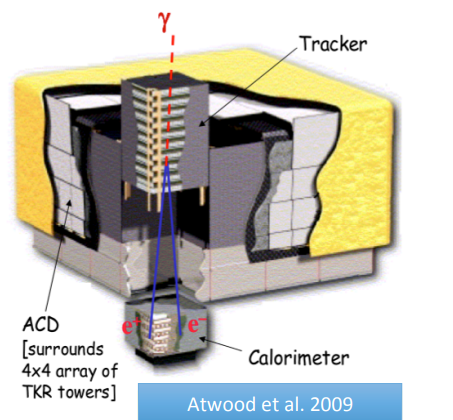
\includegraphics[scale=0.45]{PNGs/Estructura.png}
    \caption{Estructura interna del LAT}
    \label{fig:placeholder}
\end{figure}

\subsection{Fermitools}


Este es el paquete oficial de software desarrollado por el \textit{Fermi Science Support Center} para el análisis de los datos del LAT y el GBM \cite{Fermitools2019}. Se distribuye como un paquete de Python instalable mediante \texttt{conda}, y contiene el conjunto de herramientas de línea de comandos (\texttt{gtselect}, \texttt{gtmktime}, \texttt{gtbin}, \texttt{gtlike}, entre otras) necesarias para procesar los archivos FITS obtenidos del \textit{LAT Photon, Event and Spacecraft Data Query}. Estas funciones nos permiten generar desde la selección espacial, temporal y energética de eventos, hasta el cálculo de la exposición del instrumento y el ajuste de modelos espectrales mediante métodos de máxima verosimilitud. Estas herramientas se apoyan en las IRFs descritas en la sección anterior para convertir los conteos de fotones detectados en magnitudes físicas como flujos, espectros y curvas de luz \cite{FSSCCicerone}. El detalle específico de cada función utilizada se describe en la sección de Metodología.
\section{Metodología}

Para el análisis de cada uno de los GRBs estudiados en este trabajo (GRB 080916C y GRB 251118A) se siguió el flujo de trabajo estándar recomendado por el \textit{Fermi Science Support Center} para el análisis de datos del LAT \cite{FSSCCicerone}, el cual combina un análisis \textit{binned} (para caracterizar la fase prompt, de corta duración) y un análisis \textit{unbinned} de máxima verosimilitud (\textit{unbinned likelihood analysis}) para la emisión extendida de alta energía. Todas las gráficas de resultados de este informe se elaboraron con Python (\texttt{astropy}, \texttt{numpy} y \texttt{matplotlib}), excepto las de los ajustes espectrales en XSPEC, que se obtuvieron con la salida gráfica del propio programa. A continuación se presenta con más detalle el paso a paso que se realizó para el análisis de estos dos GRBs.

\subsection{Obtención de los datos}

El primer paso consiste en obtener los datos crudos del LAT a través del \textit{LAT Photon, Event, and Spacecraft Data Query} del FSSC. Para esto, es necesario que especifiquemos los siguientes parámetros de búsqueda: la posición del GRB en coordenadas ecuatoriales (RA, Dec), el radio de la región de interés (\textit{Region of Interest}, ROI), el tiempo de inicio y finalización del intervalo de interés en Tiempo del Instrumento (\textit{Mission Elapsed Time}, MET), y el rango de energía mínima y máxima en MeV. Como resultado de esta consulta se obtienen dos archivos en formato FITS: el archivo de eventos (\textit{Event file}, FT1), que contiene la lista de los eventos reconstruidos como candidatos a fotón —``evento'' en el sentido de la sección 2.2— con su tiempo de llegada, energía y dirección, y el archivo de la nave espacial (\textit{Spacecraft file}, FT2), que registra hacia dónde apuntaba el telescopio y con qué orientación durante todo el intervalo. Esa información de apuntamiento, combinada con las IRFs, es la que después permite calcular la exposición.

\subsection{Selección inicial de eventos (\texttt{gtselect})}

Aunque los archivos ya vienen recortados por la consulta, esa descarga es solo un recorte grueso: un cono espacial y una ventana de tiempo y energía sobre los datos extendidos, que traen todas las clases de eventos mezcladas. Los cortes finos se hacen en esta etapa con \texttt{gtselect}, que aplica criterios espaciales, temporales, energéticos y de calidad sobre el archivo original. Aquí se utiliza un radio de ROI relativamente amplio (típicamente de 15$^{\circ}$, holgado también frente a la incertidumbre de la posición reportada en la circular) y no se fija aún la posición exacta del centro, con el fin de contar con suficientes fotones para una localización precisa posterior de la fuente. Se aplica además un corte en el ángulo cenital (\texttt{zmax}, que en este trabajo fue de 100$^{\circ}$) para excluir fotones provenientes del limbo terrestre, y es en este paso —no en el servidor— donde se elige la clase de eventos (\texttt{evclass}) según la fase de análisis: la clase \texttt{TRANSIENT} para la emisión prompt, de mayor sensibilidad a GRBs cortos y débiles pero mayor contaminación de rayos cósmicos o fotones generados por interacción con la nave, o la clase \texttt{SOURCE}, más estricta en la discriminación del fondo, pero más sensible para GRBs de cientos de segundos.

Las llamadas completas a cada herramienta, con todos sus parámetros, se recogen en el Anexo~\ref{anexo:comandos} para no interrumpir la lectura; en el texto se citan solo los parámetros que definen cada decisión. La de \texttt{gtselect} es la del Anexo~\ref{an:gtselect}.

\subsection{Curva de luz preliminar (\texttt{gtbin})}

Con el archivo filtrado se genera una curva de luz preliminar utilizando \texttt{gtbin} en modo \texttt{LC} (\textit{Light Curve}), agrupando los eventos en bins temporales de duración fija (\texttt{dtime}). La curva se grafica con Python, con el tiempo en el eje horizontal y el número de conteos por bin en el eje vertical, lo que permite identificar visualmente la duración aproximada del estallido y su estructura temporal (Anexo~\ref{an:lc}).

\subsection{Localización de la fuente (\texttt{gtfindsrc})}

Con el objetivo de refinar la posición del GRB proporcionada inicialmente (usualmente proveniente de la localización del GBM o de una circular GCN), se utiliza \texttt{gtfindsrc}. Esta herramienta realiza un ajuste iterativo que maximiza la verosimilitud de un modelo de fuente puntual única en función de su posición, partiendo de una posición semilla y usando las IRFs (sección 2.2) correspondientes a la fase de emisión analizada. El resultado es una posición mejorada (RA, Dec) que se utiliza en los pasos subsiguientes del análisis (Anexo~\ref{an:gtfindsrc}).

\subsection{Mapa de conteos (\texttt{gtbin})}

Con la posición refinada se genera un mapa de conteos bidimensional (\texttt{CMAP}) mediante \texttt{gtbin}, en coordenadas celestes ecuatoriales (J2000). El mapa se grafica con Python para inspeccionar la distribución espacial de los eventos alrededor de la posición del GRB y confirmar visualmente que hay un exceso de conteos en la posición de la fuente.

\subsection{Definición del modelo de la región de interés}

Antes de proceder con el ajuste espectral, es necesario definir un modelo de la región de interés (ROI) en formato XML. Este modelo incluye, como mínimo, tres componentes: (i) una fuente puntual (\textit{Point Source}) ubicada en la posición refinada del GRB, con un espectro tipo ley de potencia (\texttt{PowerLaw2}); (ii) una componente de emisión difusa galáctica, que representa la emisión de rayos gamma producida por la interacción de rayos cósmicos con el gas interestelar de la Vía Láctea, modelada a partir del mapa estándar \texttt{gll\_iem\_v07.fits}, construido con el código de propagación de rayos cósmicos GALPROP (de ahí el nombre con el que esta componente aparece en los resultados); y (iii) una componente isotrópica, que representa el fondo difuso extragaláctico y el fondo residual de partículas cargadas mal clasificadas. Los archivos de fondo difuso estándar se obtienen a través del \textit{Model Editor} del FSSC, herramienta que genera automáticamente el archivo XML con la estructura y los parámetros iniciales adecuados para cada componente.

Fermitools permite escribir la ley de potencia de la fuente puntual de dos maneras, que describen la misma forma espectral y solo se diferencian en cómo se fija su normalización \cite{FSSCCicerone}. En \texttt{PowerLaw}, la normalización es un prefactor, es decir, el número de fotones por unidad de energía, de área y de tiempo a una energía de referencia (en este trabajo, 100~MeV). En \texttt{PowerLaw2}, en cambio, la normalización es directamente el flujo de fotones integrado entre dos energías (aquí, de 100~MeV a 300~GeV), de modo que el ajuste entrega el flujo y su error sin cálculos adicionales. Por esa razón el análisis se hizo con \texttt{PowerLaw2}, y \texttt{PowerLaw} se usó solo como control.

\subsection{Cálculo de la contribución difusa (\texttt{gtdiffrsp})}

Una vez definido el modelo XML de la región de interés, se ejecuta \texttt{gtdiffrsp}, la cual calcula la respuesta del instrumento a las componentes difusas del modelo para cada fotón individual: la integral del modelo difuso, convuelta con la PSF y el área efectiva, evaluada en la dirección, la energía y el tiempo de llegada de ese fotón (por eso el cálculo es fotón por fotón). El resultado se agrega como nuevas columnas (\texttt{DIFRSP0}, \texttt{DIFRSP1}, \dots) en el archivo de eventos. Este paso es indispensable para que el ajuste de máxima verosimilitud posterior pueda distinguir correctamente entre la contribución de la fuente puntual y la de los fondos difusos (Anexo~\ref{an:gtdiffrsp}).

\subsection{Livetime cube y mapa de exposición}

Posteriormente se calcula el \textit{livetime cube} con \texttt{gtltcube}, el cual almacena el tiempo efectivo de observación acumulado para cada posición del cielo, en función del ángulo con que esa posición incide respecto al eje del instrumento, a lo largo de todo el intervalo analizado (es una propiedad de cómo apuntó el telescopio, no de la fuente). A partir de este cubo se genera, mediante \texttt{gtexpmap}, un mapa de exposición: la integral del área efectiva por el tiempo efectivo de observación en cada punto y energía de la ROI, con unidades de cm$^2\,$s. La exposición es el factor que convierte flujos en conteos esperados, y por eso es indispensable para el ajuste espectral.

\subsection{Análisis binned: espectro y ajuste en XSPEC}

Para la fase prompt se realiza un análisis \textit{binned} tradicional: al ser corta y brillante, hay conteos suficientes para agruparlos por energía y ajustar el espectro acumulado (la emisión extendida, con pocos fotones repartidos en mucho tiempo, se trata con el método \textit{unbinned} de la sección 3.10). En primer lugar se genera el espectro de conteos observado con \texttt{gtbin} en modo \texttt{PHA1}, que produce un único espectro acumulado sobre toda la ventana en formato PHA (el formato estándar de espectros en astronomía de rayos X), definiendo los bordes de energía en escala logarítmica. A continuación se genera la matriz de respuesta espectral (RSP) correspondiente con \texttt{gtrspgen}, utilizando el método de cálculo \texttt{PS} (\textit{Point Source}), recomendado sobre el método \texttt{GRB} por ofrecer una mayor precisión, en particular para estallidos de mayor duración; para estallidos cortos la diferencia entre ambos métodos, tanto en resultados como en tiempo de ejecución, es despreciable. La matriz conecta dos mallas de energía distintas: la de la energía verdadera del fotón incidente, que se define en \texttt{gtrspgen}, y la de los canales del archivo PHA, que corresponden a la energía reconstruida. Como la resolución en energía del instrumento es finita, conviene que la primera malla sea más fina que la segunda (en este trabajo, 100 bins frente a 30 canales): así el número esperado de fotones en cada canal se calcula con mayor precisión (Anexo~\ref{an:binned}).

Con el espectro y su respuesta ya generados, se procede al ajuste en \texttt{XSPEC}, empleando un modelo de ley de potencia simple (\texttt{pow}). Al definir este modelo, \texttt{XSPEC} solicita como valores iniciales el índice fotónico (\texttt{PhoIndex}) y la normalización (\texttt{norm}) de la ley de potencia. El ajuste se realiza minimizando la estadística de Cash (\texttt{cstat}), apropiada para el régimen de bajo número de conteos característico de la emisión de alta energía del LAT, y se inspeccionan visualmente tanto el espectro ajustado como los residuos normalizados por su incertidumbre (Anexo~\ref{an:xspec}).

\subsection{Análisis unbinned: ajuste de máxima verosimilitud (\texttt{gtlike})}

Finalmente se analiza la emisión extendida; extendida en el tiempo: en muchos GRBs los fotones de alta energía no llegan en el pico del estallido, sino repartidos a lo largo de cientos de segundos. Para esta fase se usa el análisis de máxima verosimilitud \textit{unbinned}, en el que la verosimilitud se evalúa fotón por fotón en lugar de agrupar los eventos en bins; al no agrupar no se pierde información, y por eso es el método apropiado cuando los fotones detectados son pocos. El intervalo temporal es más amplio que el de la fase prompt y se emplea la clase \texttt{SOURCE} con su IRF (\texttt{P8R3\_SOURCE\_V3}), más estricta en la discriminación del fondo. El flujo de trabajo repite, sobre este nuevo intervalo, la selección de eventos (\texttt{gtselect}), el filtrado de calidad mediante \texttt{gtmktime} —aplicando la máscara \texttt{(DATA\_QUAL>0)\&\&(LAT\_CONFIG==1)}, que es la que el FSSC recomienda en el Cicerone para quedarse solo con datos de buena calidad y el instrumento en configuración científica \cite{FSSCCicerone}—, el cálculo de la respuesta difusa (\texttt{gtdiffrsp}, ahora con la IRF de \texttt{SOURCE}), y la generación del livetime cube y del mapa de exposición correspondientes a este nuevo intervalo, también con esa IRF (Anexo~\ref{an:extendida}).

Con todos estos archivos generados (evento filtrado, livetime cube, mapa de exposición y modelo XML), se ejecuta el ajuste de máxima verosimilitud propiamente dicho mediante la herramienta \texttt{gtlike}, en modo \texttt{UNBINNED} (el método fotón por fotón recién descrito) y con el optimizador \texttt{MINUIT} \cite{James1975}. Esta herramienta ajusta simultáneamente los parámetros libres de todas las componentes del modelo XML (la fuente puntual del GRB, la componente galáctica y la componente extragaláctica) maximizando la función de verosimilitud. La verosimilitud es la probabilidad de haber observado exactamente los datos que se observaron si el modelo fuera cierto, vista como función de los parámetros del modelo: ajustar por máxima verosimilitud es buscar los valores de los parámetros que hacen esa probabilidad lo más alta posible. En el caso \textit{unbinned} se construye como el producto, sobre todos los fotones observados, de la densidad de conteos que el modelo predice en la energía, posición y tiempo de llegada de cada uno, multiplicado por el término de Poisson del número total de conteos esperado \cite{Mattox1996} (la llamada, en el Anexo~\ref{an:gtlike}).

Como resultado de este ajuste, \texttt{gtlike} produce un archivo de salida (\texttt{.dat}) que reporta, para cada componente del modelo, los valores ajustados de sus parámetros espectrales junto con su incertidumbre estadística, el número de fotones predichos (\texttt{Npred}), el flujo integrado en el rango de energía analizado, y en el caso de la fuente puntual, el valor del estadístico de prueba (\textit{Test Statistic}, TS), definido como $\mathrm{TS} = -2\,\ln(\mathcal{L}_{0}/\mathcal{L}_{1})$, donde $\mathcal{L}_{0}$ y $\mathcal{L}_{1}$ son las verosimilitudes máximas del modelo nulo (sin la fuente) y del modelo que incluye la fuente puntual, respectivamente \cite{Mattox1996}. Este valor de TS es el criterio estándar para cuantificar la detección de un GRB con el LAT. El TS no es en sí la significancia: por el teorema de Wilks, cuando el modelo agrega un parámetro libre, la significancia aproximada en unidades de $\sigma$ es $\sqrt{\mathrm{TS}}$, y de ahí viene la regla práctica de que $\mathrm{TS} \gtrsim 25$ corresponde aproximadamente a una detección de $5\sigma$. Con pocos fotones esta aproximación es solo orientativa.
\section{Resultados}

\subsection{GRB 080916C: validación del flujo de análisis}

Antes de abordar un evento débil conviene comprobar que todo el flujo de trabajo funciona sobre uno en el
que no haya lugar a dudas. Para eso se usó el GRB 080916C, uno de los estallidos más brillantes que el
LAT ha registrado y el caso de estudio del tutorial oficial de Fermitools. Los datos se solicitaron al
servidor del FSSC en un cono de 40$^{\circ}$ alrededor de la posición inicial (RA $=121.8^{\circ}$,
Dec $=-61.3^{\circ}$), en una ventana de $\sim$2500~s alrededor del disparo
($T_0 = 243216766.614$~s MET) y entre 100~MeV y 300~GeV. Tras el filtrado con \texttt{gtselect}
(clase \texttt{TRANSIENT}, \texttt{zmax} $=100^{\circ}$), la herramienta \texttt{gtfindsrc} refinó la
posición a (RA, Dec) $=(119.861, -56.581)$, que es la que se usó en el resto del análisis.

\begin{figure}[h!]
    \centering
    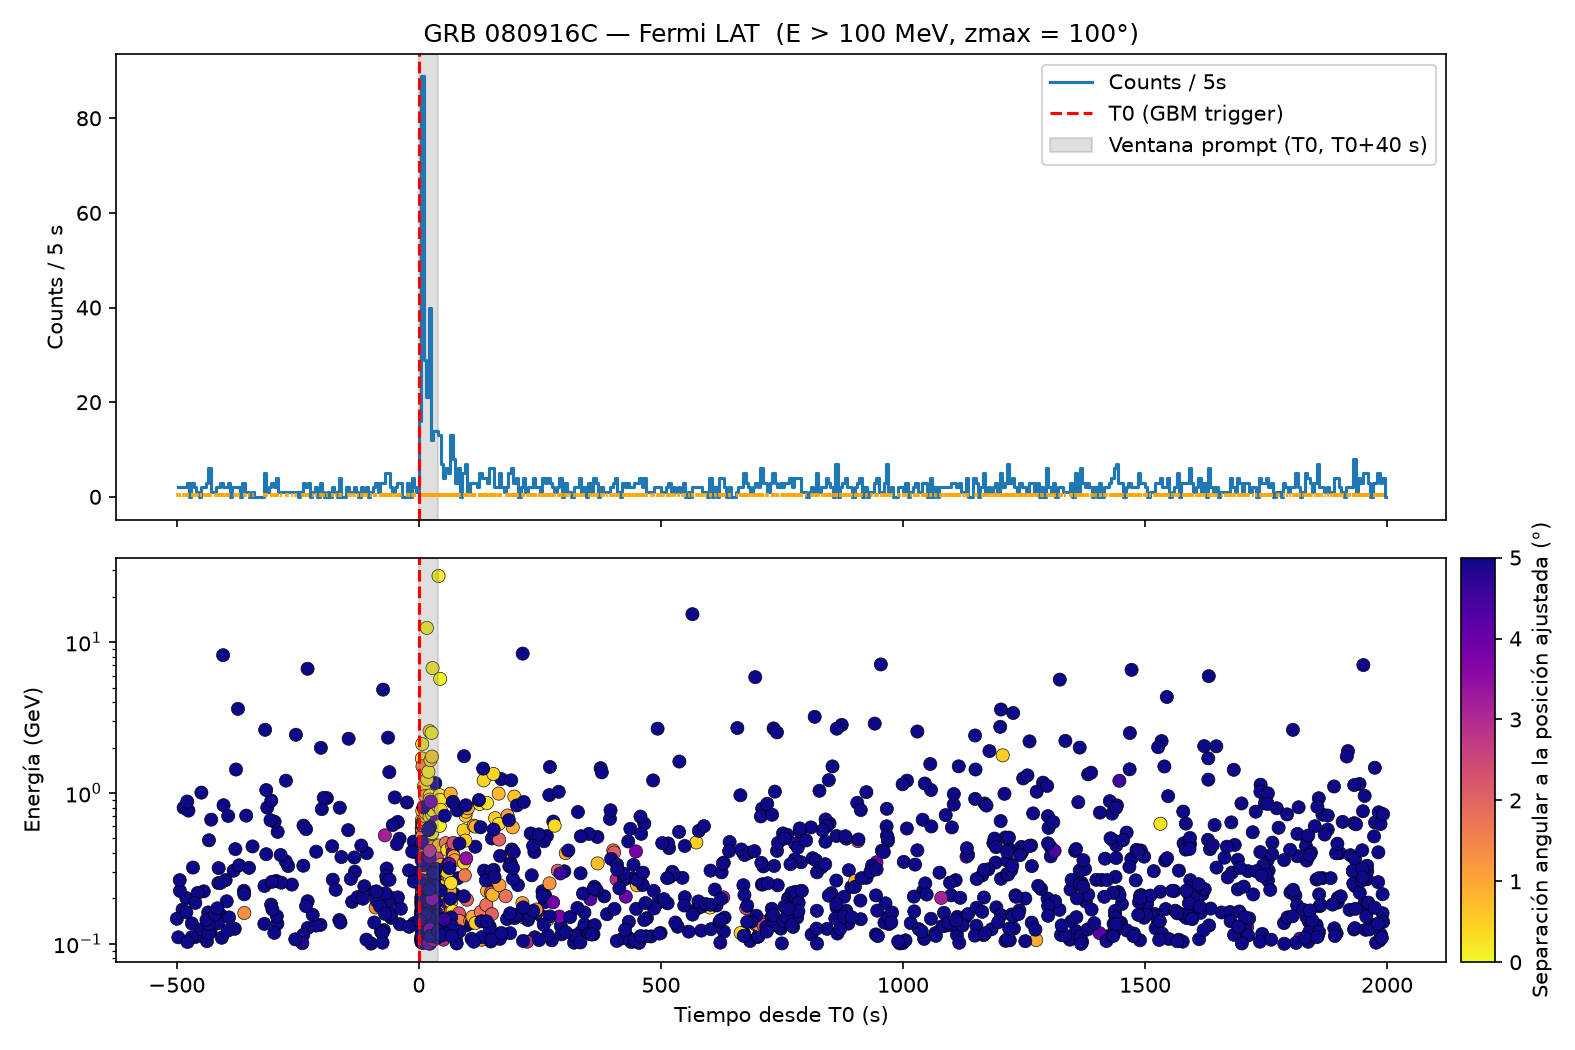
\includegraphics[width=0.95\textwidth]{PNGs/LC_080916C.png}
    \caption{Curva de luz del GRB 080916C en la banda del LAT ($E>100$~MeV, corte \texttt{zmax} $=100^{\circ}$).
    El panel superior muestra los conteos en bins de 5~s, con una marca naranja por cada fotón y la ventana
    de la fase prompt ($T_0$ a $T_0+40$~s) sombreada en gris. El panel inferior muestra la energía de cada
    fotón contra su tiempo de llegada, con el color indicando la separación angular respecto a la posición
    ajustada: los fotones más cercanos a la fuente (colores claros) se concentran en la ventana prompt,
    donde el estallido domina por completo la región.}
    \label{fig:lc080916C}
\end{figure}

La fase prompt ($T_0$ a $T_0+40$~s) dejó 219 conteos en 37~s de exposición viva, suficientes para el
análisis \textit{binned}. El ajuste en XSPEC de una ley de potencia simple con el estadístico de Cash dio
un índice fotónico $\mathrm{PhoIndex} = 2.32 \pm 0.08$, con C-stat $=26.4$ para 28 grados de libertad
(un ajuste bueno: del orden de una unidad de estadístico por grado de libertad), del orden de los valores
reportados para la emisión de alta energía de este evento \cite{Ackermann2013}. La Figura~\ref{fig:xspec080916C}
muestra el espectro ajustado y sus residuos normalizados.

\begin{figure}[h!]
    \centering
    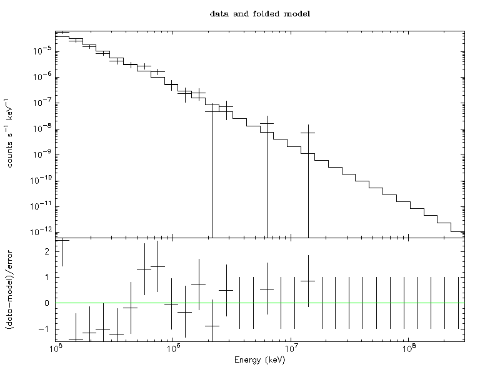
\includegraphics[width=0.75\textwidth]{PNGs/XSPEC_080916C_fit.png}
    \caption{Ajuste espectral en XSPEC de la fase prompt del GRB 080916C (modelo \texttt{powerlaw},
    estadístico de Cash). Arriba, el espectro de conteos observado y el modelo convuelto con la respuesta
    del instrumento; abajo, los residuos divididos entre la incertidumbre de cada canal, que oscilan
    alrededor de cero sin estructura: la ley de potencia simple describe bien los datos.}
    \label{fig:xspec080916C}
\end{figure}

Para la emisión extendida ($T_0+40$ a $T_0+400$~s, clase \texttt{SOURCE}) quedaron 99 fotones en la
región. El ajuste unbinned con \texttt{gtlike} dio una detección contundente:
$\mathrm{TS} = 455$ (una significancia aproximada de $\sqrt{\mathrm{TS}} \approx 21\sigma$), con índice
$\Gamma = -2.02 \pm 0.11$ y un flujo de $(6.2 \pm 0.8)\times10^{-5}$~ph~cm$^{-2}$~s$^{-1}$ entre 100~MeV
y 200~GeV. De los 99 fotones, el modelo atribuye 70.2 al GRB: incluso 40~s después del disparo, el
estallido seguía dominando la región. La Tabla~\ref{tab:resumen080916C} resume ambos ajustes y la
Figura~\ref{fig:espectro080916C} muestra el espectro de conteos con las componentes del modelo.

\begin{table}[h!]
\centering
\caption{Resumen del análisis del GRB 080916C. La fase prompt se ajustó con el método binned (XSPEC,
ley de potencia simple, estadístico de Cash) y la emisión extendida con el método unbinned
(\texttt{gtlike}). En XSPEC el índice se define positivo, $N(E)\propto E^{-\mathrm{PhoIndex}}$, de modo
que $\mathrm{PhoIndex}=2.32$ equivale a $\Gamma=-2.32$ en la convención de \texttt{gtlike}.}
\label{tab:resumen080916C}
\begin{tabular}{lcc}
\toprule
 & \textbf{Prompt (binned)} & \textbf{Extendida (unbinned)} \\
\midrule
Ventana & $T_0$ a $T_0+40$~s & $T_0+40$ a $T_0+400$~s \\
Clase de eventos & \texttt{TRANSIENT} & \texttt{SOURCE} \\
Fotones en la región & 219 & 99 \\
Índice & $\mathrm{PhoIndex} = 2.32 \pm 0.08$ & $\Gamma = -2.02 \pm 0.11$ \\
Flujo [ph~cm$^{-2}$~s$^{-1}$] & --- & $(6.2 \pm 0.8)\times10^{-5}$ \\
Bondad / detección & C-stat $= 26.4/28$ g.l. & $\mathrm{TS} = 455$ ($\approx 21\sigma$) \\
Npred (GRB) & --- & 70.2 \\
\bottomrule
\end{tabular}
\end{table}

\begin{figure}[h!]
    \centering
    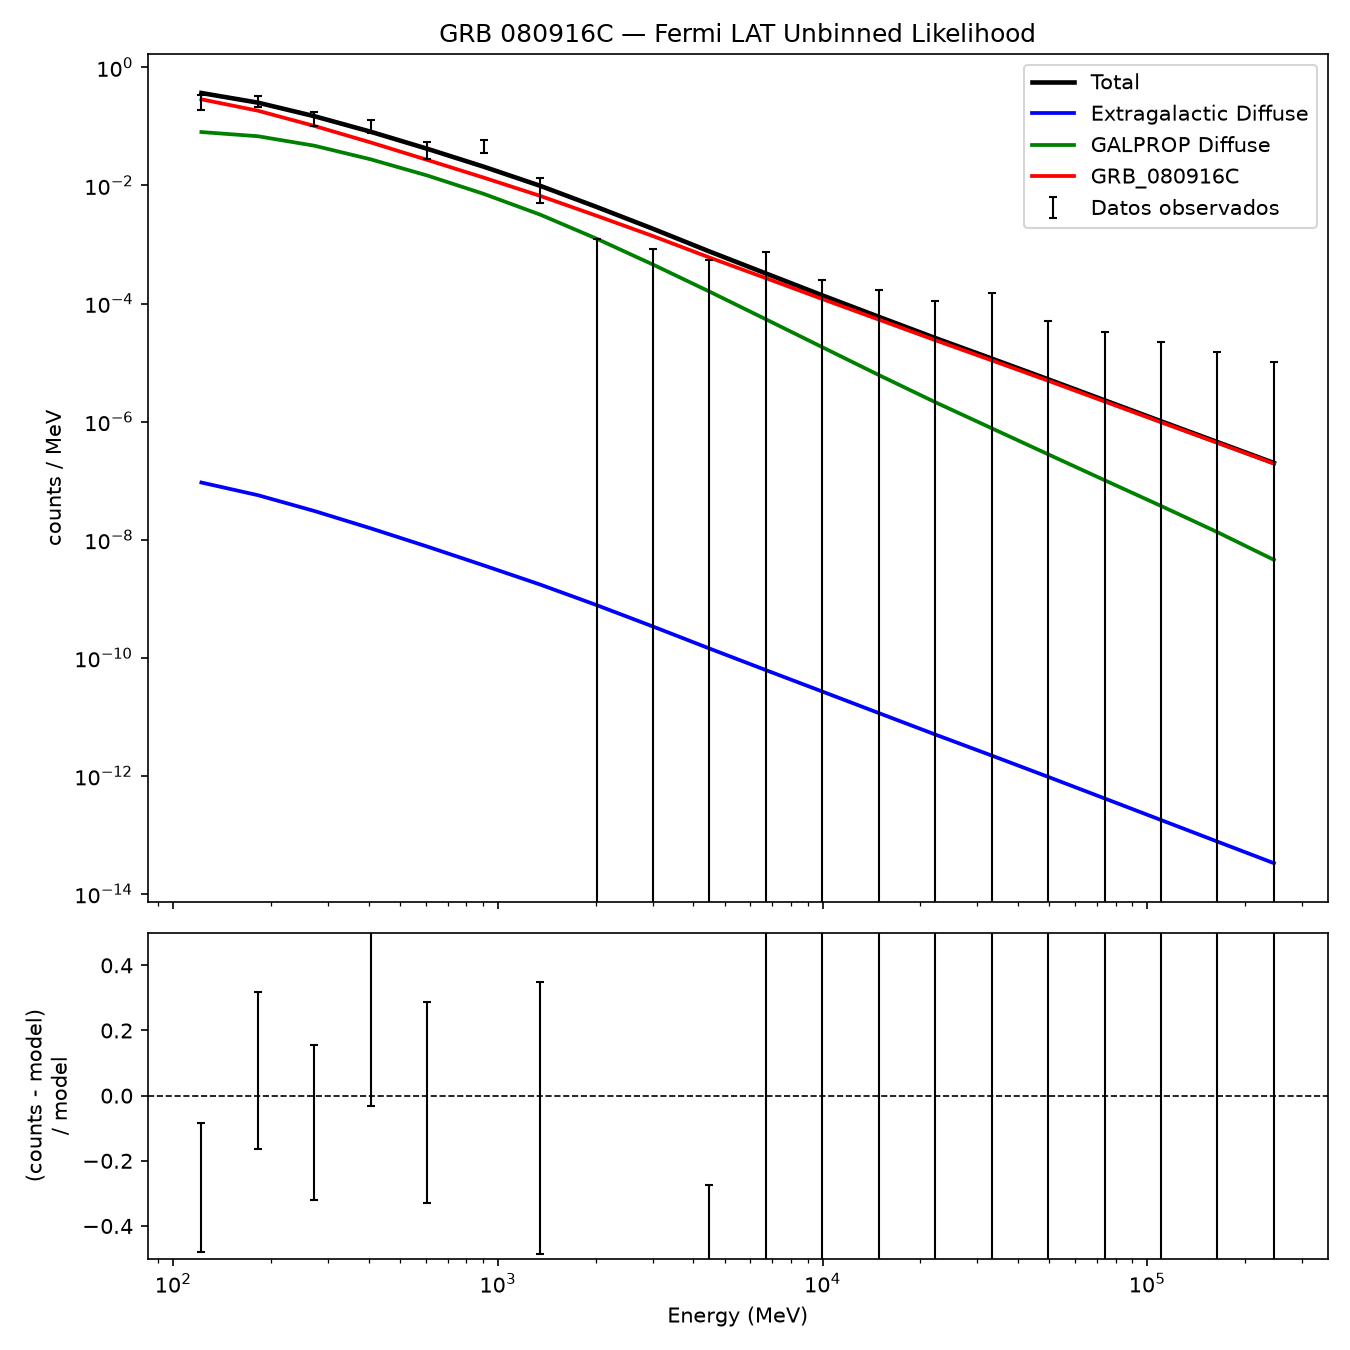
\includegraphics[width=0.8\textwidth]{PNGs/Espectro_080916C.png}
    \caption{Espectro de conteos de la emisión extendida del GRB 080916C y componentes del modelo
    ajustado con \texttt{gtlike}: en rojo la fuente puntual del GRB, en verde el difuso galáctico
    (GALPROP), en azul el difuso extragaláctico y en negro la suma, con los datos y sus barras de error
    poissonianas. El panel inferior muestra los residuos relativos (conteos $-$ modelo)/modelo. El GRB
    domina sobre los fondos en prácticamente toda la banda, como corresponde a un evento tan brillante.}
    \label{fig:espectro080916C}
\end{figure}

Un detalle del ajuste merece mención honesta: con una ventana tan corta, las dos componentes difusas del
modelo son casi degeneradas entre sí, y el ajuste llevó el prefactor del fondo isotrópico a su cota
inferior (Npred $\approx 0$) mientras la normalización galáctica subía a $2.10 \pm 0.42$. Para el
propósito de esta validación eso es inocuo —los fondos enteros aportan $\sim$29 de los 99 fotones y el
GRB está detectado a $21\sigma$ se reparta como se reparta el difuso—, pero anticipa el problema que
domina el siguiente análisis: cuando los fotones escasean, el reparto entre fuente y fondos se vuelve la
decisión central.

\subsection{GRB 251118A}

\subsubsection{Datos, posición y selección de eventos}

El GRB 251118A fue detectado por el GBM el 18 de noviembre de 2025 a las 20:31:30.09 UT
($T_0 = 785190695.09$~s MET), con $T_{90} = 46.6$~s en la banda de 50--300~keV y una fluencia de
$(1.03\pm0.01)\times10^{-4}$~erg~cm$^{-2}$ \cite{GCN42783}: en rayos gamma de baja energía fue un
estallido brillante. El LAT lo detectó y localizó en RA $=160.08^{\circ}$, Dec $=-34.58^{\circ}$
($\pm0.17^{\circ}$, 90\,\% de contención) \cite{GCN42752}, pero en condiciones adversas: al momento del
disparo la fuente estaba a $69^{\circ}$ del eje óptico del instrumento (el \textit{boresight}, la normal
al plano superior del LAT, desde donde se mide el ángulo de incidencia), casi al borde del campo de
visión útil ($\sim$70$^{\circ}$), donde el área efectiva es mínima. Eso explica que, siendo brillante en
keV, en el LAT dejara apenas unas decenas de fotones.

El seguimiento de Swift encontró el afterglow del estallido: XRT lo detectó en rayos X decayendo como
$t^{-1.08}$ \cite{GCN42782} y UVOT midió su contraparte óptica en RA $=160.00422^{\circ}$,
Dec $=-34.52254^{\circ}$ con una precisión de $0.42''$ \cite{GCN42786}, a $5'$ de la posición del LAT y
dentro de su radio de error. Esa posición de UVOT, cuya incertidumbre es despreciable frente a la PSF
del LAT, es la que se adoptó para la fuente puntual y para todas las separaciones angulares; con ella,
el paso de localización con \texttt{gtfindsrc} resulta innecesario.

Los datos se solicitaron en un cono de 30$^{\circ}$ alrededor de la posición del LAT, de $T_0-1000$ a
$T_0+3700$~s y entre 100~MeV y 300~GeV (700 eventos en la consulta). Sobre ellos se hicieron dos
selecciones con la clase \texttt{SOURCE} y \texttt{zmax} $=100^{\circ}$, ambas con radio de
15$^{\circ}$: una \textbf{ventana de análisis} de $T_0$ a $T_0+1500$~s —la misma que usa la circular del
LAT para el flujo, de modo que ambos resultados sean directamente comparables—, que tras
\texttt{gtmktime} quedó con \textbf{35 fotones} en un único intervalo de buen tiempo de 1500~s, y una
\textbf{ventana larga} de $T_0-100$ a $T_0+3600$~s, solo para la curva de luz, con 39 fotones en 2512~s
de buen tiempo. La Tabla~\ref{tab:radios251118A} muestra cómo se reparten los fotones de la ventana de
análisis según la distancia a la posición del GRB.

\begin{table}[h!]
\centering
\caption{Fotones de la ventana de análisis del GRB 251118A ($T_0$ a $T_0+1500$~s, clase \texttt{SOURCE},
\texttt{zmax} $=100^{\circ}$) según el radio de extracción medido desde la posición del afterglow de
UVOT. La concentración hacia radios pequeños —5 fotones dentro de $1^{\circ}$— ya sugiere una fuente
puntual sobre un fondo repartido por toda la región.}
\label{tab:radios251118A}
\begin{tabular}{lc}
\toprule
\textbf{Radio de extracción} & \textbf{Fotones} \\
\midrule
$< 15^{\circ}$ & 35 \\
$< 10^{\circ}$ & 18 \\
$< 5^{\circ}$  & 9 \\
$< 2^{\circ}$  & 5 \\
$< 1^{\circ}$  & 5 \\
$< 0.5^{\circ}$ & 3 \\
\bottomrule
\end{tabular}
\end{table}

\subsubsection{Curva de luz y nivel de fondo}

La Figura~\ref{fig:lc251118A} muestra la curva de luz de la ventana larga en bins de 50~s, junto con la
energía y la separación angular de cada fotón. Los cinco fotones que llegaron a menos de 1$^{\circ}$ de
la posición del afterglow lo hicieron a los 279, 578, 1239, 1394 y 1457~s después del disparo, mucho
después de que terminara la emisión prompt registrada por el GBM, cuyo $T_{90}$ de 46.6~s aparece como
una banda gris en la figura. La emisión que detectó el LAT no corresponde entonces a la cola del
estallido en keV, sino a una fase posterior. El aumento de conteos que se observa entre $\sim$400 y
$\sim$700~s se debe, en cambio, a fotones que llegaron lejos de la posición del GRB y que corresponden
en su mayoría al fondo.

Entre esos cinco fotones está el de mayor energía de la ventana, de 6.8~GeV, que llegó a
$T_0+1394$~s y se reconstruyó a solo 0.05$^{\circ}$ de la posición del afterglow. Se trata del mismo
fotón que reporta la circular del LAT \cite{GCN42752}, y su cercanía a esa posición es la indicación más
directa, previa a cualquier ajuste, de que los datos contienen emisión del GRB.

Después de $\sim$1500~s no llegó ningún fotón a la región. Entre $T_0+2000$ y $T_0+3600$~s el
instrumento acumuló solo 412~s de buen tiempo, porque el barrido del cielo sacó la región del campo de
visión, de modo que la ausencia de fotones en ese intervalo es consistente con el apagado de la fuente,
pero no alcanza para medir la tasa de fondo. Por esa razón, el fondo se estima con el modelo del ajuste
de máxima verosimilitud que se presenta en las secciones siguientes.

\begin{figure}[h!]
    \centering
    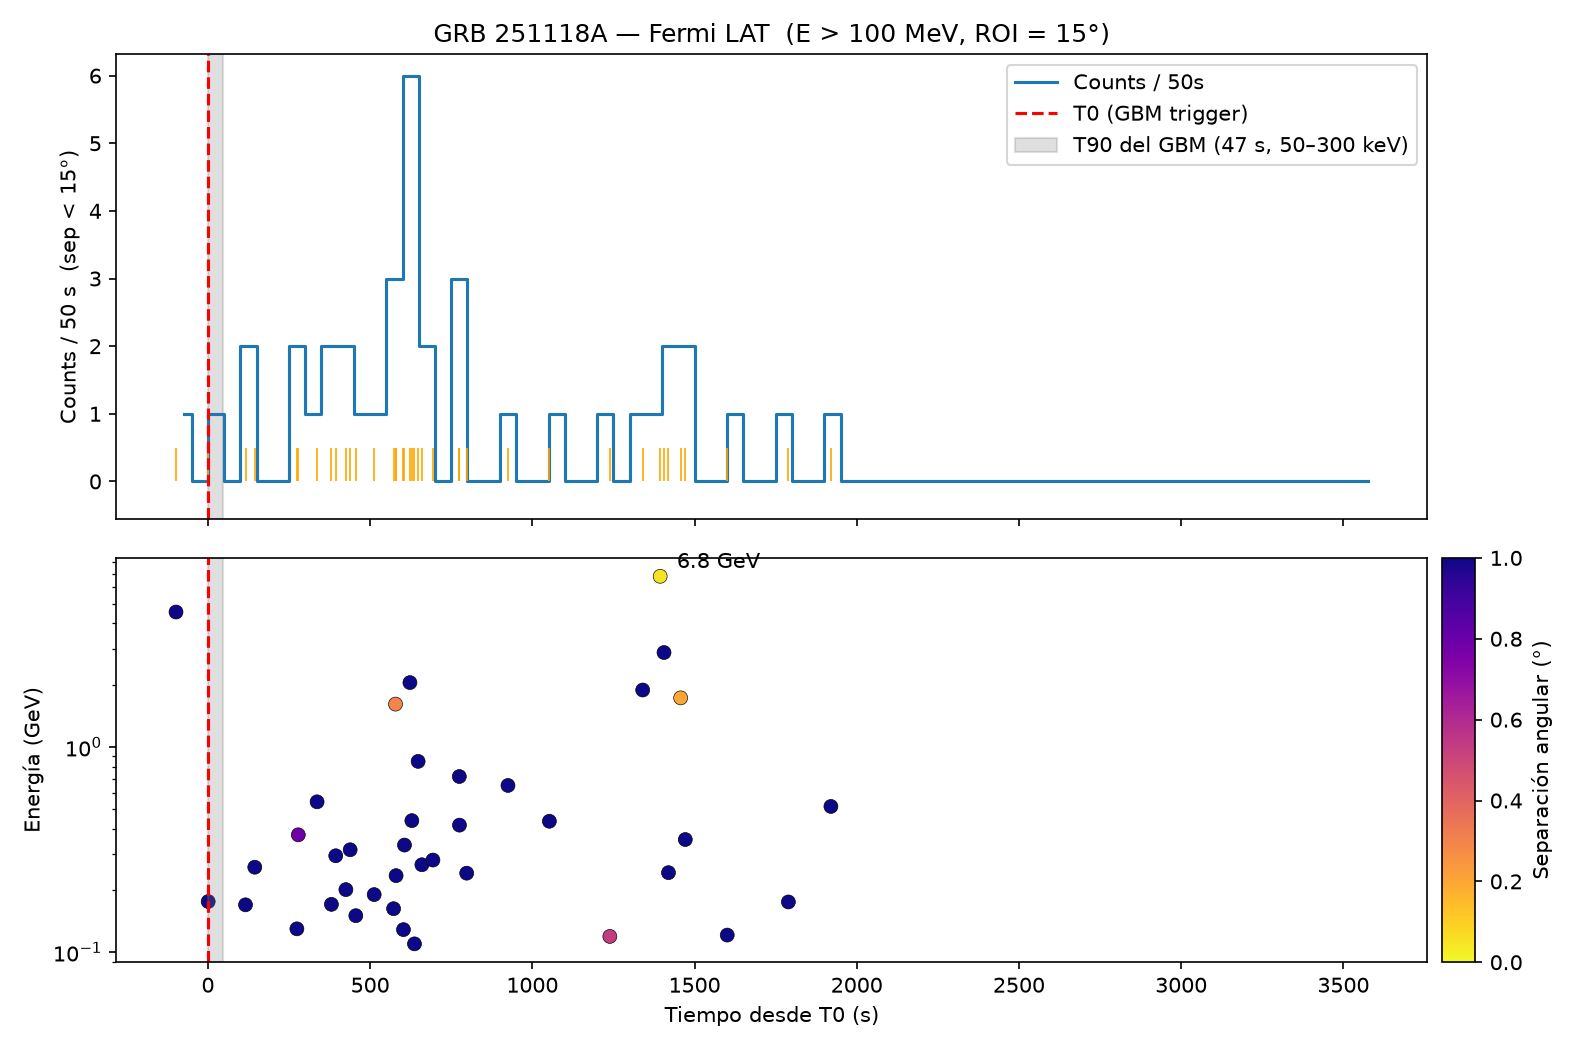
\includegraphics[width=0.95\textwidth]{PNGs/LC_251118A_larga.png}
    \caption{Curva de luz del GRB 251118A en la banda del LAT ($E>100$~MeV, radio de 15$^{\circ}$),
    de $T_0-100$ a $T_0+3600$~s. El panel superior muestra los conteos en bins de 50~s y una marca
    naranja por cada fotón, y la banda gris corresponde al $T_{90}$ del GBM (46.6~s, 50--300~keV). El
    panel inferior muestra la energía de cada fotón contra su tiempo de llegada, y el color indica su
    separación angular respecto a la posición del afterglow, desde amarillo (sobre la fuente) hasta azul
    oscuro (1$^{\circ}$ o más). El fotón de 6.8~GeV, que llegó a $T_0+1394$~s, aparece prácticamente
    sobre la posición del afterglow.}
    \label{fig:lc251118A}
\end{figure}

\subsubsection{Modelo de la región y variantes del ajuste}

El modelo de la región tiene las tres componentes descritas en la Metodología, que son la fuente puntual
del GRB en la posición del afterglow, con un espectro de ley de potencia (\texttt{PowerLaw2}), el difuso
galáctico (GALPROP) y el fondo isotrópico. El prefactor y el índice del fondo isotrópico se dejaron fijos
en sus valores de catálogo, porque con 35 fotones el ajuste se vuelve inestable cuando todas las
normalizaciones quedan libres y la matriz de covarianza deja de ser definida positiva.

El GRB se encuentra a una latitud galáctica de $b = 21^{\circ}$ y la región de interés tiene un radio de
15$^{\circ}$, por lo que el plano galáctico queda fuera de ella y la contribución galáctica proviene de
la emisión difusa a latitudes medias. El modelo tampoco incluye las fuentes puntuales del catálogo 4FGL
que hay dentro de la región. Su aporte en 1500~s es muy pequeño comparado con el de los fondos difusos,
pero su omisión es una limitación de este análisis.

Cuando hay tan pocos fotones, la decisión de modelado que más influye en el resultado es cuáles
parámetros se fijan y cuáles se dejan libres. Para examinarla se ajustaron cuatro variantes del mismo
modelo sobre los mismos datos, descritas en la Tabla~\ref{tab:variantes251118A}, y cada par de variantes
difiere en una sola decisión. La comparación entre V1 y V2 muestra el efecto de fijar la normalización
galáctica en su valor nominal de 1. La comparación entre V2 y V3 muestra el efecto de fijar además el
índice del GRB en el valor de la circular ($-1.8$), algo que solo es posible porque este GRB ya cuenta con
una circular y que no podría hacerse con un evento nuevo. Por último, la comparación entre V4 y V1 sirve
como control, ya que \texttt{PowerLaw} y \texttt{PowerLaw2} son la misma ley de potencia escrita de dos
maneras y deberían dar el mismo resultado.

\begin{table}[h!]
\centering
\caption{Las cuatro variantes del modelo ajustadas al GRB 251118A. La columna ``Espectro GRB'' indica cuál de
las dos formas de la ley de potencia descritas en la Metodología se usó para la fuente puntual. La
última columna enumera los parámetros que quedaron libres en todo el modelo, incluida la normalización
galáctica cuando no está fija.}
\label{tab:variantes251118A}
\small
\setlength{\tabcolsep}{4.5pt}
\begin{tabular}{lllll}
\toprule
\textbf{Variante} & \textbf{Índice GRB} & \textbf{GALPROP} & \textbf{Espectro GRB} & \textbf{Parámetros libres} \\
\midrule
V1 & libre & libre & \texttt{PowerLaw2} & Integral, Index, Value (3) \\
V2 & libre & fija $=1$ & \texttt{PowerLaw2} & Integral, Index (2) \\
V3 & fijo $=-1.8$ & fija $=1$ & \texttt{PowerLaw2} & Integral (1) \\
V4 & libre & libre & \texttt{PowerLaw} & Prefactor, Index, Value (3) \\
\bottomrule
\end{tabular}
\end{table}

\subsubsection{Ajuste de máxima verosimilitud}

La Tabla~\ref{tab:gtlike251118A} presenta los resultados de las cuatro variantes. Como las variantes
tienen distinto número de parámetros libres, sus valores de TS no se comparan directamente. La
significancia de cada una se calculó a partir de su TS y del número de parámetros libres que corresponden
al GRB, que son dos en V1, V2 y V4 (el flujo y el índice) y uno en V3 (solo el flujo). Solo en este último
caso la significancia coincide con $\sqrt{\mathrm{TS}}$.

\begin{table}[h!]
\centering
\caption{Resultados del ajuste unbinned del GRB 251118A para las cuatro variantes del modelo
(ventana $T_0$ a $T_0+1500$~s, radio de 15$^{\circ}$). Se reportan el número de parámetros libres de todo
el modelo, el TS con su significancia aproximada (calculada con los parámetros libres del GRB), el índice
y el flujo del GRB con sus errores a 1$\sigma$, el número de fotones que el modelo atribuye al GRB
(Npred) y la normalización ajustada del difuso galáctico. El isotrópico quedó fijo en sus valores de
catálogo en todas las variantes y aporta Npred $=9.4$.}
\label{tab:gtlike251118A}
\small
\setlength{\tabcolsep}{4.5pt}
\begin{tabular}{lcccccc}
\toprule
\textbf{Var.} & \textbf{Parám.} & \textbf{TS} ($\approx\sigma$) & \textbf{Índice} ($\Gamma$) & \textbf{Flujo [$10^{-6}$~ph~cm$^{-2}$~s$^{-1}$]} & \textbf{Npred} & \textbf{GALPROP} \\
\midrule
V1 & 3 & 42.7 (6.2$\sigma$) & $-1.77 \pm 0.30$ & $2.08 \pm 1.02$ & 7.4 & $1.26 \pm 0.34$ \\
V2 & 2 & 46.0 (6.5$\sigma$) & $-1.80 \pm 0.30$ & $2.22 \pm 1.03$ & 7.8 & 1 (fija) \\
V3 & 1 & 46.0 (6.8$\sigma$) & $-1.8$ (fijo) & $2.22 \pm 0.90$ & 7.8 & 1 (fija) \\
V4 & 3 & 42.7 (6.2$\sigma$) & $-1.77 \pm 0.30$ & $2.08 \pm 2.29$ & 7.4 & $1.26 \pm 0.34$ \\
\bottomrule
\end{tabular}
\end{table}

Al fijar la normalización galáctica en 1 (de V1 a V2), el TS sube de 42.7 a 46.0 y el índice queda
prácticamente en el valor de la circular. Cuando la normalización se deja libre, como en V1, converge a
$1.26 \pm 0.34$. Ese valor es compatible con 1 dentro de su error, pero tiende a crecer porque absorbe
fotones que de otro modo se atribuirían al GRB, de modo que con esta cantidad de fotones conviene fijarla
en su valor nominal.

Fijar además el índice del GRB (de V2 a V3) no cambia el TS, que se mantiene en 46.0, y su único efecto
es reducir el error del flujo de 1.03 a 0.90 ($\times10^{-6}$~ph~cm$^{-2}$~s$^{-1}$). Esa reducción es
la que se espera al quitar un parámetro libre y no representa una mejora física del ajuste. La variante
V4, por su parte, reproduce el TS y el índice de V1, lo que confirma que el cambio de parametrización no
altera el resultado. La diferencia en el error del flujo de V4 se debe a que en esa parametrización el
flujo no es un parámetro del ajuste, y su error se propaga desde el prefactor, que está fuertemente
correlacionado con el índice.

Por estas razones se adopta V2 como resultado del análisis, ya que mide el índice con los datos propios
en lugar de tomarlo de la circular y mantiene el fondo galáctico en su valor nominal. Con esta variante
se obtiene $\mathrm{TS} = 46.0$, que con dos parámetros libres del GRB equivale a unas 6.5$\sigma$, un
índice $\Gamma = -1.80 \pm 0.30$ y un flujo de $(2.22 \pm 1.03)\times10^{-6}$~ph~cm$^{-2}$~s$^{-1}$ por
encima de 100~MeV.

El mismo ajuste permite estimar cuánto fondo hay en la región. De los 35 fotones observados, el modelo
atribuye 16.1 al difuso galáctico, 9.4 al isotrópico y 7.8 al GRB, para un total predicho de 33.2
fotones. Cerca de tres de cada cuatro fotones de la región corresponden entonces al fondo, y la señal del
GRB se reduce a unos ocho fotones, lo que explica buena parte de la dificultad de este análisis. La
Figura~\ref{fig:espectro251118A} muestra el espectro de conteos con este reparto entre componentes.

\begin{figure}[h!]
    \centering
    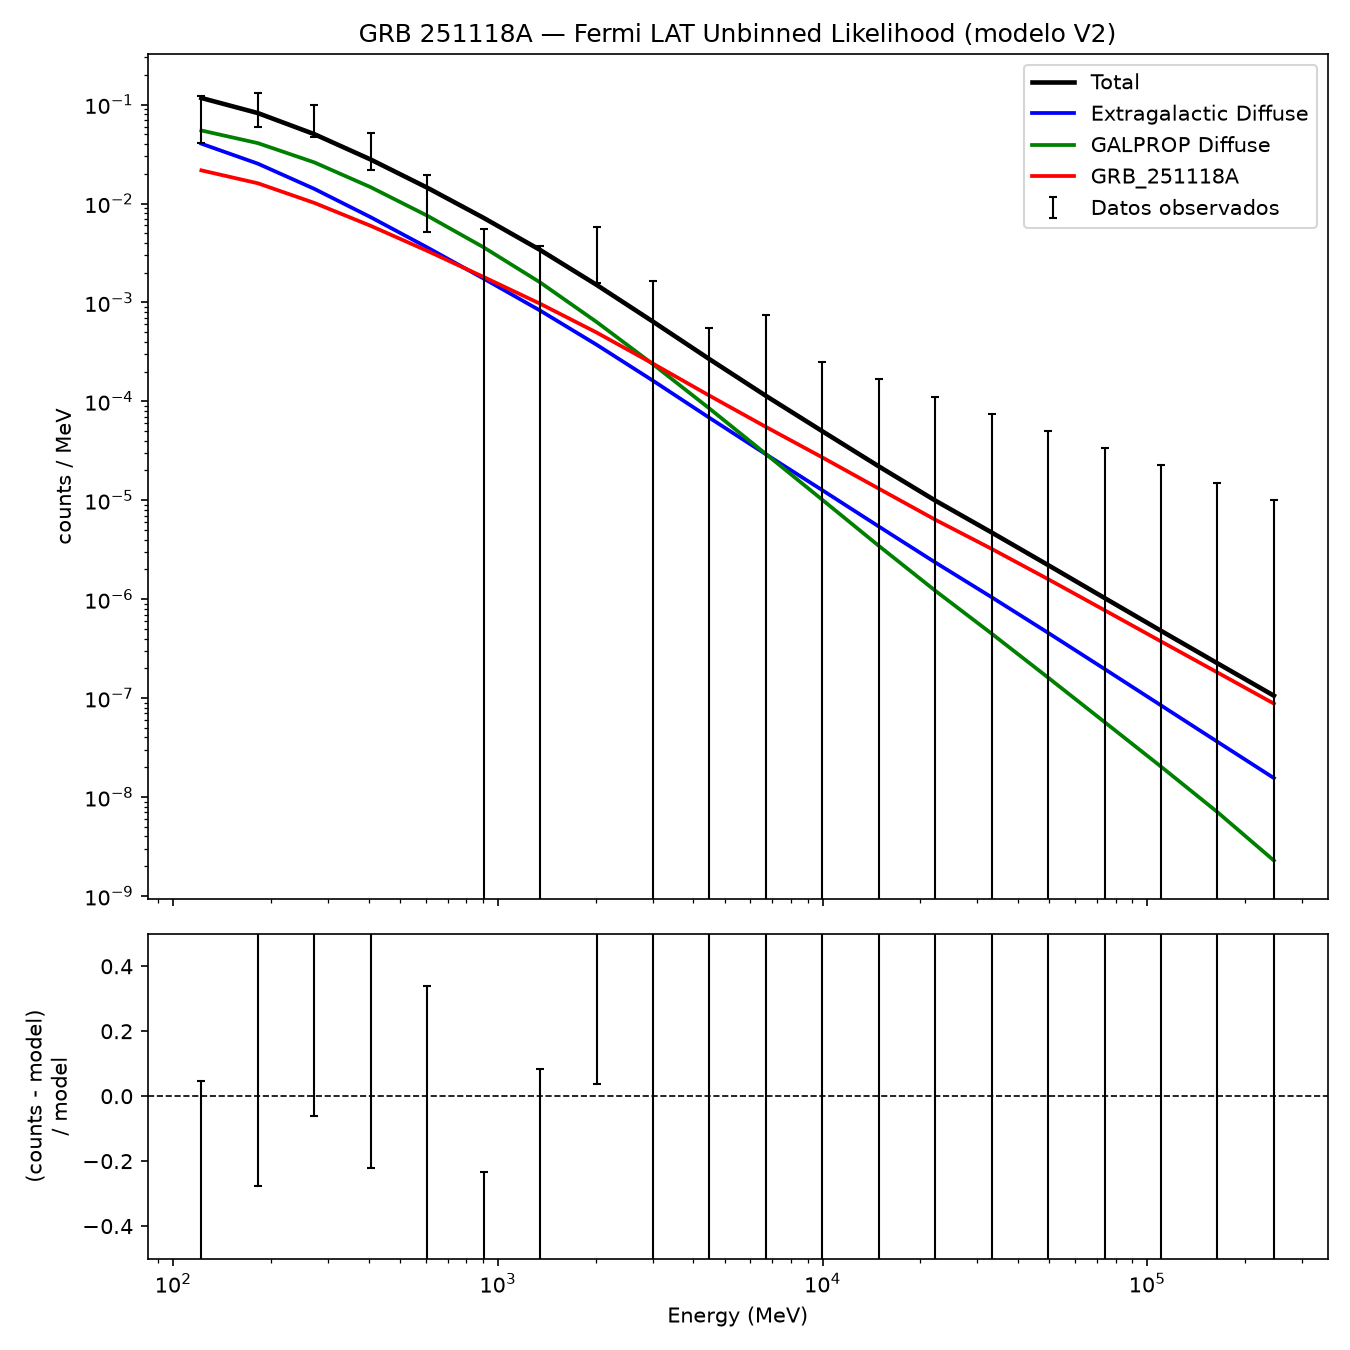
\includegraphics[width=0.82\textwidth]{PNGs/Espectro_251118A_V2.png}
    \caption{Espectro de conteos del GRB 251118A y componentes del modelo V2 ajustado con
    \texttt{gtlike}. El GRB aparece en rojo, el difuso galáctico (GALPROP) en verde, el isotrópico en
    azul y la suma en negro, junto con los datos y sus barras de error poissonianas, y el panel inferior
    muestra los residuos relativos. Por debajo de $\sim$1~GeV dominan los fondos difusos, que concentran
    la mayoría de los 35 fotones. Entre 1 y 2~GeV el GRB se vuelve comparable al fondo galáctico, y por
    encima de unos pocos GeV domina la región, por lo que el fotón de 6.8~GeV tiene un peso grande en la
    detección.}
    \label{fig:espectro251118A}
\end{figure}

\subsubsection{Verificación con el análisis binned}

Como control independiente se construyó también el espectro binned de la misma ventana, con 30 canales
logarítmicos en energía, y se ajustó en XSPEC una ley de potencia simple con el estadístico de Cash. El
ajuste dio $\mathrm{PhoIndex} = 1.98 \pm 0.17$, con un C-stat de 13.2 para 28 grados de libertad
(Figura~\ref{fig:xspec251118A}).

Este control tiene una limitación importante. El ajuste binned no incluye un modelo de fondo, por lo que
su ley de potencia describe el total de fotones de la región, es decir, el GRB junto con los cerca de 25
fotones de los fondos difusos, y no al GRB por separado. Por eso, que su índice quede a 0.5$\sigma$ del
índice del GRB obtenido en el ajuste unbinned indica únicamente que la forma espectral del conjunto es
coherente con la del GRB. La medición del GRB propiamente dicha es la del ajuste unbinned.

XSPEC reporta además, junto al ajuste, una probabilidad nula que se calcula con la estadística
$\chi^{2}$. Ese valor no es interpretable en este caso, porque con 35 fotones repartidos en 30 canales la
mayoría de los canales tiene 0, 1 o 2 conteos y la estadística $\chi^{2}$ deja de ser válida. Por esa
razón, la bondad del ajuste se evalúa con el C-stat en relación con sus grados de libertad.

\begin{figure}[h!]
    \centering
    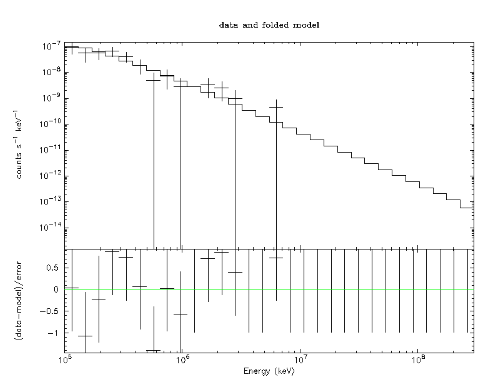
\includegraphics[width=0.75\textwidth]{PNGs/XSPEC_251118A_fit.png}
    \caption{Ajuste espectral binned del GRB 251118A en XSPEC (modelo \texttt{powerlaw}, estadístico de
    Cash) sobre la ventana de análisis completa. El panel superior muestra el espectro de conteos y el
    modelo convolucionado con la respuesta del instrumento, y el inferior los residuos divididos entre la
    incertidumbre de cada canal. Las barras de error grandes corresponden a canales con 0 o 1 conteos, algo
    inevitable con 35 fotones en 30 canales. Aun así, los residuos no muestran una estructura sistemática y
    la ley de potencia describe bien el conjunto.}
    \label{fig:xspec251118A}
\end{figure}

\subsubsection{Comparación con la circular GCN y lectura física}

Para decidir si dos mediciones coinciden no basta con comparar sus valores centrales. Es necesario
dividir su diferencia entre la incertidumbre combinada, $|x_1-x_2|/\sqrt{\sigma_1^{2}+\sigma_2^{2}}$, y
se considera que dos valores son consistentes cuando el resultado es menor que 2. La
Tabla~\ref{tab:comparacion251118A} aplica este criterio a los resultados de este trabajo y a los de la
circular del LAT \cite{GCN42752}. Conviene tener presente que ambas mediciones se hicieron con los mismos
fotones, de manera que no son independientes y la incertidumbre combinada sirve solo como una medida
orientativa del acuerdo.

\begin{table}[h!]
\centering
\caption{Comparación de los resultados del GRB 251118A con la circular GCN 42752, en unidades de la
incertidumbre combinada ($\sigma$ comb.). El índice de XSPEC se expresa en la convención de
\texttt{gtlike} ($\Gamma = -\mathrm{PhoIndex}$). Su flujo no se reporta porque la normalización de XSPEC
no es directamente un flujo de fotones y, al no haber modelo de fondo, correspondería al total de la
región.}
\label{tab:comparacion251118A}
\small
\setlength{\tabcolsep}{4.5pt}
\begin{tabular}{lcccc}
\toprule
\textbf{Análisis} & \textbf{Índice} ($\Gamma$) & $\sigma$ \textbf{comb.} & \textbf{Flujo [$10^{-6}$~ph~cm$^{-2}$~s$^{-1}$]} & $\sigma$ \textbf{comb.} \\
\midrule
Unbinned, V2 (este trabajo) & $-1.80 \pm 0.30$ & 0.0 & $2.22 \pm 1.03$ & 0.3 \\
Binned, XSPEC (este trabajo) & $-1.98 \pm 0.17$ & 0.5 & --- & --- \\
GCN 42752 & $-1.8 \pm 0.3$ & --- & $1.8 \pm 0.7$ & --- \\
\bottomrule
\end{tabular}
\end{table}

El índice obtenido coincide con el de la circular, con una diferencia de 0.0$\sigma$, y el flujo difiere
en 0.3$\sigma$. El valor central del flujo es ligeramente mayor que el de la circular, una diferencia que
cabe dentro de la fluctuación de Poisson que se espera cuando la señal es de unos ocho fotones. El
control binned queda a 0.5$\sigma$ de ambos índices. Hay que considerar que la circular proviene del
análisis automático de la colaboración, calibrado con cientos de GRB, por lo que el hecho de que este
análisis manual la reproduzca valida el flujo de trabajo aprendido, que era el objetivo de la práctica.

En cuanto a la interpretación física, la emisión prompt registrada por el GBM terminó en unos 47~s y su
espectro, descrito por una función de Band, tiene en la parte de alta energía un índice
$\beta = -2.56 \pm 0.06$ \cite{GCN42783}. El LAT, en cambio, registró fotones hasta unos 1500~s después
del disparo, con un índice $\Gamma = -1.80 \pm 0.30$, es decir, un espectro más duro que la cola de alta
energía del prompt, con una diferencia de 2.5$\sigma$ combinadas. La llegada tardía de los fotones y su
espectro más duro apuntan a que la emisión GeV del GRB 251118A no es una extrapolación del prompt, sino
una componente distinta y posterior, consistente con el afterglow temprano que Swift-XRT observó decaer
como $t^{-1.08}$ \cite{GCN42782}. Como no se ha reportado un corrimiento al rojo para este evento, no es
posible convertir estos flujos en energía isotrópica.

\newpage
\begin{center}
\section*{Conclusiones}
\end{center}

\begin{itemize}
\setlength{\itemsep}{0.4cm}

\item Se preparó y verificó el entorno necesario para analizar GRB con datos del LAT. Se instaló Fermitools mediante conda en el entorno \texttt{fermi}, junto con XSPEC (v12.15.1) y las bibliotecas de Python con las que se leyeron los archivos FITS y se elaboraron las gráficas (\texttt{astropy}, \texttt{numpy} y \texttt{matplotlib}). Las pruebas realizadas comprobaron el funcionamiento de las herramientas y la disponibilidad de los archivos de calibración y de los modelos de fondo, con lo que se contó con un entorno funcional para trabajar con datos reales del LAT.

\item La reproducción del análisis del GRB 080916C permitió comprobar que el entorno funcionaba correctamente antes de aplicarlo a un evento distinto. Se siguió el flujo completo del tutorial oficial de Fermitools, desde la selección y preparación de los datos hasta el ajuste de máxima verosimilitud con \texttt{gtlike} y el análisis espectral con XSPEC. Por tratarse de un GRB ampliamente estudiado y con resultados disponibles en la literatura, este caso sirvió para aprender el procedimiento y verificar que las herramientas funcionaban en conjunto. El ajuste binned de la fase prompt dio un índice $\mathrm{PhoIndex} = 2.32 \pm 0.08$ y el ajuste unbinned de la emisión extendida dio una detección con $\mathrm{TS}=455$ y $\Gamma = -2.02 \pm 0.11$, valores del mismo orden que los reportados en la literatura para este evento.

\item El análisis del GRB 251118A permitió aplicar el flujo completo de trabajo a un evento real, desde la descarga y selección de los datos hasta el análisis espectral y de máxima verosimilitud. Entre los fotones de la ventana de análisis se identificó el fotón de 6.8~GeV reportado en la circular, reconstruido a solo 0.05$^{\circ}$ de la posición del afterglow. El ajuste de máxima verosimilitud dio una detección con $\mathrm{TS}=46.0$, equivalente a unas 6.5$\sigma$, un índice $\Gamma = -1.80 \pm 0.30$ y un flujo de $(2.22\pm1.03)\times10^{-6}$~ph~cm$^{-2}$~s$^{-1}$, que difieren de los valores de la circular GCN en 0.0 y 0.3 incertidumbres combinadas, respectivamente. El ajuste binned de control en XSPEC ($\mathrm{PhoIndex} = 1.98 \pm 0.17$) quedó a 0.5$\sigma$ de ambos índices.

\item Las variantes del modelo mostraron que, cuando se dispone de pocos fotones, el tratamiento del fondo galáctico es la decisión que más influye en el resultado. Fijar su normalización en el valor nominal subió el TS de 42.7 a 46.0, mientras que fijar también el índice espectral no cambió el TS y solo redujo el error del flujo, como se espera al quitar un parámetro libre.

\item El trabajo quedó documentado en este informe, que incluye el procedimiento seguido, los fundamentos de las herramientas utilizadas, las decisiones metodológicas, los problemas encontrados y la interpretación de los resultados principales. Su elaboración permitió organizar el proceso completo del análisis y dejar registro de lo aprendido durante las prácticas, desde la preparación del entorno hasta el estudio del GRB 251118A. Los cuadernos de Jupyter con el flujo completo de ambos análisis, ya ejecutados, están disponibles en un repositorio público\footnote{\url{https://github.com/USUARIO/REPOSITORIO}}.

\item En conjunto, las prácticas permitieron pasar de la configuración inicial de las herramientas a un análisis completo de un GRB con datos del LAT, con resultados para el GRB 251118A consistentes con los publicados en la GCN 42752. Además del uso de Fermitools, XSPEC y las distintas etapas del procesamiento de datos, el análisis mostró la importancia de las decisiones metodológicas, en especial del tratamiento del fondo cuando se trabaja con pocos fotones. Esta experiencia ofrece una base práctica para continuar con el análisis de GRB y de otros fenómenos transitorios en la astrofísica de altas energías.

\end{itemize}

\newpage
\appendix
\section{Llamadas a las herramientas de Fermitools}
\label{anexo:comandos}

Este anexo recoge las llamadas completas a cada herramienta utilizada en el análisis, en el orden en que
aparecen en la Metodología. Cada línea corresponde a un parámetro de la herramienta (archivo de entrada,
archivo de salida, cortes, etc.); los valores entre \texttt{<~>} dependen del GRB analizado y se indican
en la sección de Resultados.

\subsection{Selección inicial de eventos}
\label{an:gtselect}

\begin{lstlisting}[style=mipython]
gtselect \
  infile=<archivo_de_eventos>.fits \
  outfile=<archivo_filtrado>.fits \
  ra=INDEF \
  dec=INDEF \
  rad=15 \
  tmin=<MET_inicio> \
  tmax=<MET_fin> \
  emin=100 \
  emax=300000 \
  zmax=100 \
  evclass=16
\end{lstlisting}

\subsection{Curva de luz}
\label{an:lc}

\begin{lstlisting}[style=mipython]
gtbin \
  algorithm=LC \
  evfile=<archivo_filtrado>.fits \
  outfile=<curva_de_luz>.fits \
  scfile=<archivo_de_nave>.fits \
  tstart=<MET_inicio> \
  tstop=<MET_fin> \
  dtime=<ancho_del_bin> \
  tbinalg=LIN
\end{lstlisting}

\subsection{Localización de la fuente}
\label{an:gtfindsrc}

\begin{lstlisting}[style=mipython]
gtfindsrc \
  evfile=<archivo_filtrado>.fits \
  scfile=<archivo_de_nave>.fits \
  outfile=<resultado_localizacion>.txt \
  irfs=P8R3_TRANSIENT020_V3 \
  coordsys=CEL \
  ra=<RA_semilla> \
  dec=<Dec_semilla> \
  optimizer=MINUIT
\end{lstlisting}

\subsection{Contribución difusa}
\label{an:gtdiffrsp}

\begin{lstlisting}[style=mipython]
gtdiffrsp \
  evfile=<archivo_filtrado>.fits \
  scfile=<archivo_de_nave>.fits \
  srcmdl=<modelo>.xml \
  irfs=<IRF_de_la_fase>
\end{lstlisting}

\subsection{Espectro de conteos y matriz de respuesta (análisis binned)}
\label{an:binned}

\begin{lstlisting}[style=mipython]
gtbin \
  algorithm=PHA1 \
  evfile=<archivo_filtrado>.fits \
  outfile=<espectro>.pha \
  scfile=<archivo_de_nave>.fits \
  ebinalg=LOG \
  emin=100 \
  emax=300000 \
  enumbins=30

gtrspgen \
  respalg=PS \
  specfile=<espectro>.pha \
  scfile=<archivo_de_nave>.fits \
  outfile=<respuesta>.rsp \
  thetacut=90 \
  dcostheta=0.5 \
  irfs=CALDB \
  ebinalg=LOG \
  emin=100 \
  emax=300000 \
  enumbins=100
\end{lstlisting}

\subsection{Ajuste espectral en XSPEC}
\label{an:xspec}

\begin{lstlisting}[style=mipython]
xspec
query yes
data <espectro>.pha
model pow
    <PhoIndex inicial>
    <norm inicial>
statistic cstat
cpd /xs
setplot energy
fit
plot ldata delchi
show all
\end{lstlisting}

\subsection{Preparación de la ventana extendida}
\label{an:extendida}

\begin{lstlisting}[style=mipython]
gtselect evclass=128 \
  infile=<FT1>.fits \
  outfile=<seleccion_extendida>.fits \
  ra=<RA> \
  dec=<Dec> \
  rad=15 \
  tmin=<MET_inicio_ext> \
  tmax=<MET_fin_ext> \
  emin=100 \
  emax=300000 \
  zmax=100

gtmktime \
  scfile=<FT2>.fits \
  filter="(DATA_QUAL>0)&&(LAT_CONFIG==1)" \
  roicut=yes \
  evfile=<seleccion_extendida>.fits \
  outfile=<mktime_extendida>.fits

gtdiffrsp \
  evfile=<mktime_extendida>.fits \
  scfile=<FT2>.fits \
  srcmdl=<modelo>.xml \
  irfs=P8R3_SOURCE_V3

gtltcube \
  evfile=<mktime_extendida>.fits \
  scfile=<FT2>.fits \
  outfile=<ltcube_extendida>.fits \
  dcostheta=0.025 \
  binsz=0.5

gtexpmap \
  evfile=<mktime_extendida>.fits \
  scfile=<FT2>.fits \
  expcube=<ltcube_extendida>.fits \
  outfile=<expmap_extendida>.fits \
  irfs=P8R3_SOURCE_V3
\end{lstlisting}

\subsection{Ajuste de máxima verosimilitud}
\label{an:gtlike}

\begin{lstlisting}[style=mipython]
gtlike \
  statistic=UNBINNED \
  results=<resultados>.dat \
  scfile=<FT2>.fits \
  evfile=<mktime_extendida>.fits \
  expmap=<expmap_extendida>.fits \
  expcube=<ltcube_extendida>.fits \
  srcmdl=<modelo>.xml \
  irfs=P8R3_SOURCE_V3 \
  optimizer=MINUIT
\end{lstlisting}






\newpage
\bibliographystyle{unsrtnat}  
\bibliography{ref}            

\end{document}